%----------------------------------------------------------------------------------------
%	PACKAGES AND DOCUMENT CONFIGURATIONS
%----------------------------------------------------------------------------------------
\documentclass[11pt]{article}
\usepackage{amsmath} % Required for some math elements
\usepackage{hyperref} 
\usepackage{xcolor}
\usepackage{lipsum} 
\usepackage{cite}
\usepackage{graphicx} % Required for the inclusion of images
\usepackage{algorithmic}
\usepackage{array}
\usepackage{bookmark}
\usepackage{listings}
\usepackage{amssymb}
\usepackage{enumitem}
\usepackage[margin=24mm]{geometry}
\usepackage[caption=false, font=footnotesize]{subfig}
\usepackage{multirow}
\usepackage[active,tightpage]{preview}

\renewcommand{\PreviewBorder}{1in}
\newcommand{\Newpage}{\end{preview}\begin{preview}}

\newlist{steps}{enumerate}{1}
\setlist[steps, 1]{label = Step \roman*:}

\hypersetup{ %color attributes of citation, link, etc.
    colorlinks=true,
    linkcolor=blue,
    filecolor=gray,      
    urlcolor=blue,
    citecolor=blue,
}

\newcommand{\matlab}{\textsc{Matlab }} %very important and totally necessary addition

\newcommand\Item[1][]{%
  \ifx\relax#1\relax  \item \else \item[#1] \fi
  \abovedisplayskip=0pt\abovedisplayshortskip=0pt~\vspace*{-\baselineskip}}
  %----------------------------------------------------------------------------------------
%	DOCUMENT INFORMATION
%----------------------------------------------------------------------------------------
 
\title{ECEN303 : Test 2 \\ Circuits, Op amp limitations, Noise, Stability, Oscillators}
\author{Daniel Eisen : 300447549}
\date{\today}

\begin{document}
\begin{preview}
\maketitle
%----------------------------------------------------------------------------------------
%	DOCUMENT CONTENT
%----------------------------------------------------------------------------------------
\section*{Question 1}
\begin{enumerate}[label=\alph*)]
        \item c)
        \item c)
        \item d)
        \item c)
        \item a)
        \item a)
        \item b)
        \item a)
        \item d)
        \item c)
        \item c)
        \item a)
\end{enumerate}

\section*{Question 2}
Assume $T=25^{\circ}C,\:298.15K$:
\begin{enumerate}[label=\roman*)]
        \item   $e_{n} = \sqrt{4KTR}$\\
                $e_{R1} = e_{RP} = 4.057 nV/\sqrt{Hz}$\\
                $e_{R2} = 27.81 nV/\sqrt{Hz}$\\

        \item   $v_n=15nV/\sqrt{Hz},\:i_n=7pA/\sqrt{Hz},\:A_{+}=48,\:A_{-}=47$\\

                $R_{PN}=e_{RP}\cdot A_{+} = 194.47nV/\sqrt{Hz}$\\
                $R_{1N}=e_{R1}\cdot A_{-} = 190.67nV/\sqrt{Hz}$\\
                $R_{2N}=e_{R2} = 27.81 nV/\sqrt{Hz}$\\
                $O_{n}=v_{n}\cdot A_{+} = 720nV/\sqrt{Hz}$\\
                $i_{+}=i_{n}\cdot R_{1}\cdot A_{+} = 336nV/\sqrt{Hz}$\\
                $i_{-}=i_{n}\cdot R_{2} = 329nV/\sqrt{Hz}$\\

                Total = $\sqrt{R_{PN}^{2}+R_{1N}^{2}+R_{2N}^{2}+O_{n}^{2}+i_{+}^{2}+i_{-}^{2}} = 902.54nV/\sqrt{Hz}$

        \item   $B = 999.95$\\
                $V_{out}\:Noise = Total{\cdot}B = 902.5\mu V$
\end{enumerate}
\section*{Question 3}
\begin{enumerate}[label=\roman*)]
        \item To deal with $I_B$ we set $R_P + R_A = R_1 // R_2 = 957\Omega$\\
        To stick with standard resistor values, $R_P = 910\Omega$, $R_A = 47\Omega$\\
        Input voltage offset max: $3+(957*0.00003)=3.02871$ but allow for $\pm4mV$ of control.\\
        $\frac{V_x}{V_y} = \frac{R_A}{R_A+R_B} = \frac{4mV}{15V} \therefore R_B = \frac{47}{\frac{4\cdot10^{-3}}{15}}-47 176.2K \approx 170K$ for more control. \\
        $R_c << R_B$ thus 10K

        \item The process in time consuming and expensive, difficult to automate, the offset drift of an op amp with temperature will vary with the
        setting of its offset adjustment.

        \item Can use a programmable DAC for external trimming.
\end{enumerate}
\section*{Question 4}
\begin{enumerate}[label=\roman*)]
        \item The Vo is saturated at 1 rail, until the output crosses the threshold set be R1, R2, and then Vo snaps to the other rail.   

        \item $V_{T}=\pm0.25V,\:V_{T}=\pm0.25V$\\
        $V_T = \frac{R_1}{R_1+R_2}V_O$\\
        Choose $R_1=1K$ then $R_2=\frac{R_{1}}{\frac{V_{T}}{V_{O}}}-R_{1} = 51K$

        \item Can be used to compensate for contact switch bonusing and cutting out noise, ie for a audio noise gate. 
\end{enumerate}
\section*{Question 5}
\begin{enumerate}[label=\roman*)]
        \item The circuit has a initial stage of an half wave rectifier that is then combined at the inverting rectifier with the input at a 2:1 ratio. to get a inverted full wave rectification.
        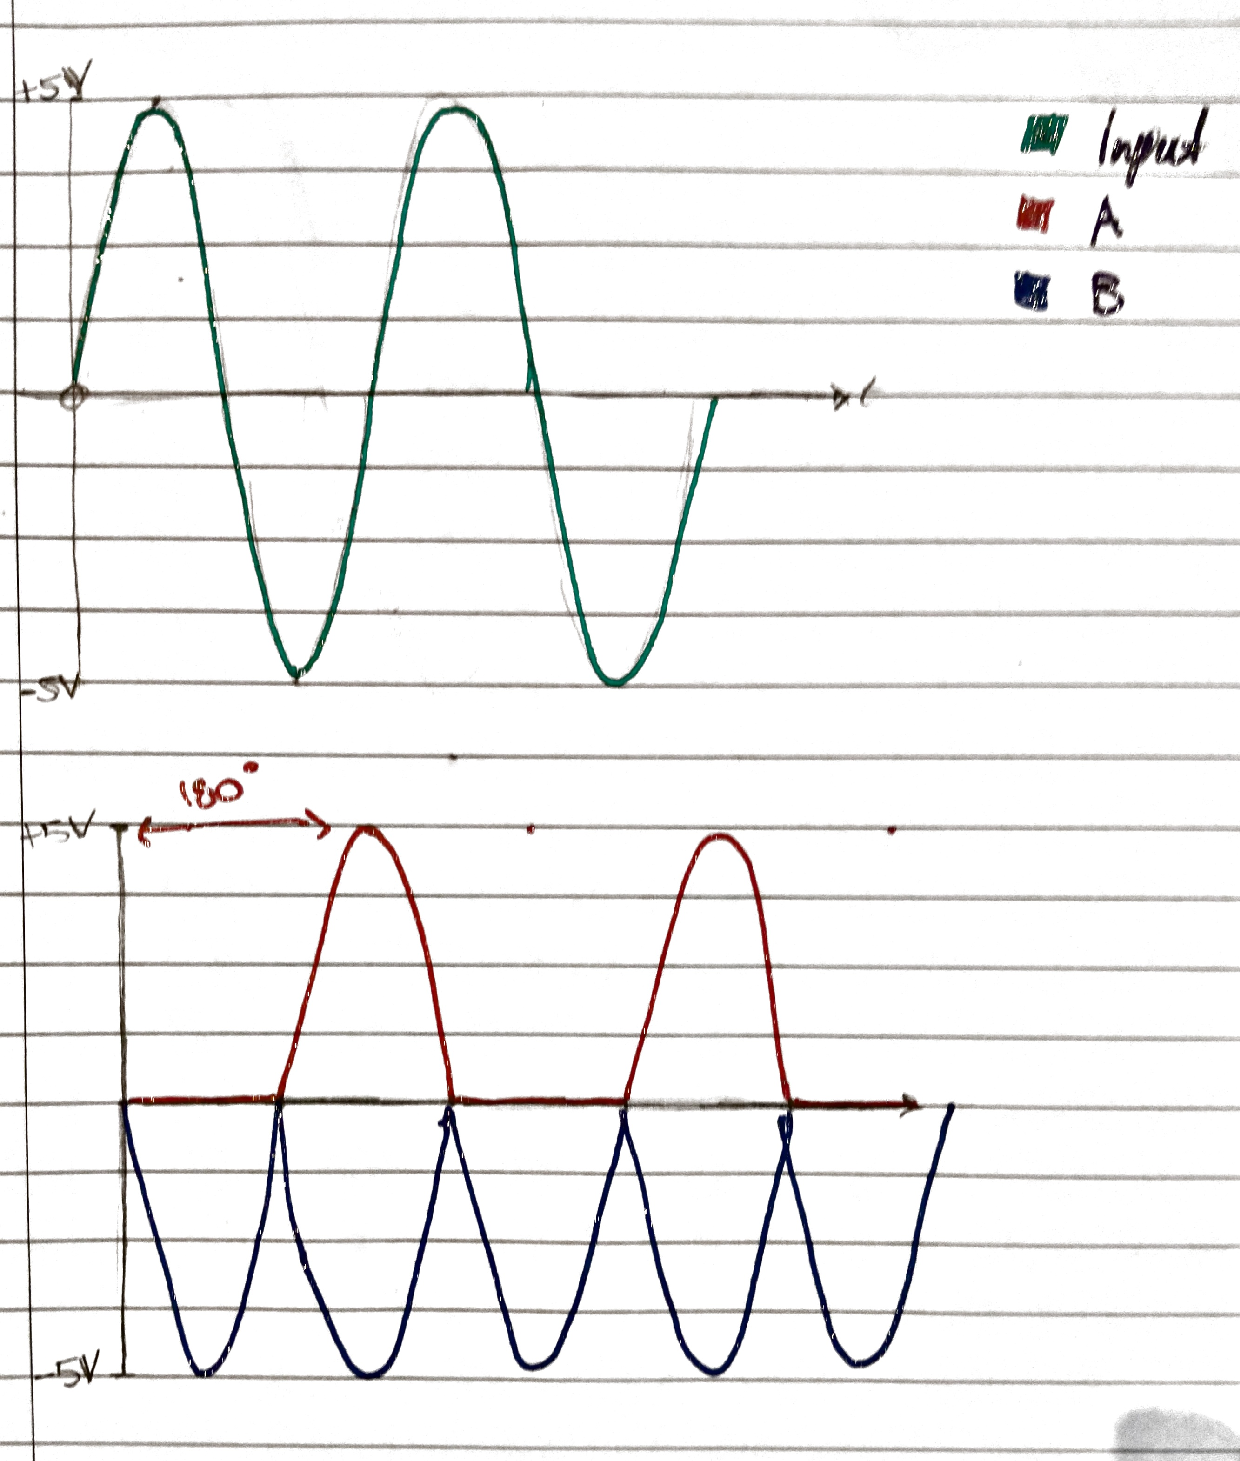
\includegraphics[width=0.67\textwidth]{5.pdf}
        
        \item This is an inverting full wave rectifier.
\end{enumerate}
\section*{Question 6}
\begin{enumerate}[label=\roman*)]
        \item This is grounding scheme that is used to prevent ground loops. It involves have components referencing the \textbf{same} point, not intermediate points.

        {\centering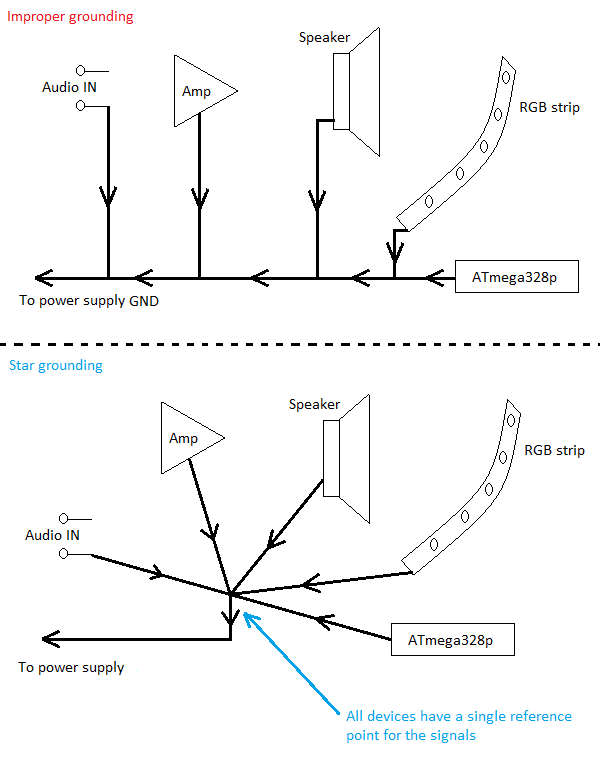
\includegraphics[width=0.42\textwidth]{star.png}\\}

        \item A pole placed at an appropriate low frequency in the open-loop response reduces the gain of the amplifier to one (0 dB) for a frequency at or just below the location of the next highest frequency pole. This is to allow  for greater open loop bandwidth while still maintaining amplifier closed loop stability.

        \item To do this we increase the phases rate of change, to do this we add poles in the form of an RC chain.
\end{enumerate}

\end{preview}
\end{document}